\documentclass[11pt]{article}
\usepackage{graphicx}

\begin{document}
	\begin{center}
		\begin{Large}
			Assignment No 6
		\end{Large}
	\end{center}•
	Aim:Code Generation using LEX and YACC.\\
	
	\noindent
	Objective:
	\begin{enumerate}
		\item To understand working of Code Generation Phase of Compiler.
		\item To generate a code using sethi-ullman algorithm..
	\end{enumerate}•
	
	\noindent
	Software Requirement:
	\begin{enumerate}
		\item Linux Operating System
		\item Lex compiler
		\item Yacc compiler
	\end{enumerate}•
	
	\noindent
	Mathematical Model:\\
	Consider a set S consisting of all the elements related to a program.The mathematical model is given as below,\\
	S={s,e,X,Y,Fme,DD,NDD,Mem shared} Where,\\ s = Initial State e = End State\\
	X	= Input data. Here it is arithmetic expression. for eg. a+b*c.\\
	Y	= Output. Here it is An assembly statements such as Mov a,R0.\\
	Fme = Algorithm/Function used in program.for eg.{createnode(),labelling(),gencode()}\\
	DD = Deterministic Data\\
	NDD = Non deterministic Data Mem shared = Memory shared by processor.\\
	
	
	\begin{center}
		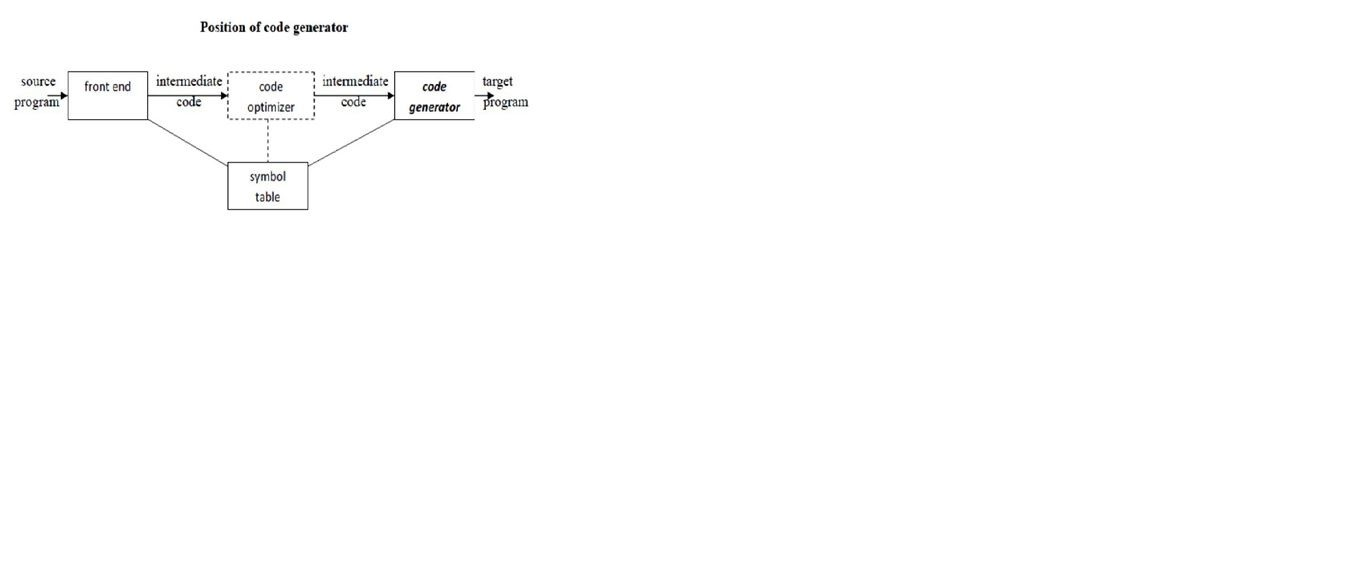
\includegraphics{te.png}
	\end{center}•
	The final phase in compiler model is the code generator. It takes as input an intermediate representation of the source program and produces as output an equivalent target program. The code generation techniques presented below can be used whether or not an optimizing phase occurs before code generation.\\
	
	\noindent
	Issues in Code Generation Phase:\\
	Following generic issues are concerned while designing code generator:\\
	\begin{enumerate}
		\item Input to the code generator:\\
		The input to the code generator consists of the intermediate representation of the source program produced by the front end, together with information in the symbol table that is used to determine the run time addresses of the data objects denoted by the names in the intermediate representation.\\
		We assume that prior to code generation the front end has scanned, parsed, and translated the source program into a reasonably detailed intermediate representation,The code generation phase can proceed on the assumption that its input is free of errors. In some compilers, this kind of semantic checking is done together with code generation.\\
		\item Target program:\\
		The output of the code generator is the target program. The output may take on a variety of forms: absolute machine language, relocatable machine language, or assembly language.\\
		\item Memory Management:\\
		Mapping names in the source program to addresses of data objects in run time memory is done cooperatively by the front end and the code generator. We assume that a name in a three-address statement refers to a symbol table entry for the name.\\
		\item Instruction Selection:\\
		For each type of three address statement, we can design a code skeleton that outlines the target code to be generated for that construct.Depending on the target machine ,instruction generation might be having uniformity and completeness.\\
		For example: x=y+z can be written as,\\
		MOV R1,z\\
		ADD R1,y\\
		MOV x,R1\\
		\item Register Allocation :\\
		Instructions involving register operands are usually shorter and faster than those involving operands in memory. Therefore, efficient utilization of registers is particularly important in generating good code. The use of registers is often subdivided into two subproblems :\\
		\begin{enumerate}
			\item During register allocation , we select the set of variables that willreside in registers at a point in the program.
			\item During a subsequent register assignment phase, we pick the specific register that a variable will reside in.
		\end{enumerate}•
		\item Evaluation Order :
		
	\end{enumerate}•
	
	Sometimes, order of evaluation also impacts the performance of system (such as efficiency of target code).\\
	
	
	\noindent
	SETHI-ULLMAN ALGORITHM FOR CODE GENERATION :\\
	The sethi-ullman code generation algorithm generates the shortest sequence of instructions.It is Provably optimal algorithm (w.r.t. length of the sequence).This algorithm is suitable for expression trees (basic block level). It is considered as a Machine model,wherein all computations are carried out in registers and instructions are of the form op R,R or op M,R. Always computes the left subtree into a register and reuses it immediately.\\
	
	\noindent
	There are two phases while generating a code using sethi-ullman algorithm.\\
	\begin{enumerate}
		\item Labelling Phase:\\
		It labels each node of the tree with an integer and fewest no. of registers require to evaluate the tree with no intermediate stores to memory.\\
		\begin{enumerate}
			\item For leaf nodes if n is the leftmost child of its parent then, label(n) := 1 else label(n) := 0
			\item For internal nodes label(n) = max (l1, l2), if l1$<>$ l2
			= l1 + 1, if l1 = l2
		\end{enumerate}•
		
		\item Code Generation Phase:\\
		Procedure gencode(n)\\
		\begin{enumerate}
			\item Case 0: if\\
			n is a leaf representingoperand N and is the leftmost child of its parent then print(LOAD N, top(RSTACK))\\
			\item Case 1: else if\\
			n is an interior node with operatorOP, left child n1, and right child n2 then\\
			if label(n2) == 0 then\\
			{
				let N be the operand for n2;\\
				gencode(n1); print(OP N, top(RSTACK));\\
			}\\
			\item Case 2: else if ((1 $<$ label(n1) $<$ label(n2)) and( label(n1) $<$ r)) then {\\
				swap(RSTACK); gencode(n2); R := pop(RSTACK); gencode(n1); /* R holds the result of n2 */ print(OP R, top(RSTACK)); push (RSTACK,R); swap(RSTACK);\\
			}
			\item Case 3: else if ((1 $<= $label(n2) $<=$ label(n1)) and( label(n2) $<$ r)) then {\\
				gencode(n1);\\
				R := pop(RSTACK); gencode(n2); /* R holds the result of n1 */ print(OP top(RSTACK), R); push (RSTACK,R);\\
			}
			\item Case 4: both labels are $>=$ r else { gencode(n2); T:= pop(TSTACK); print(LOAD top(RSTACK), T); gencode(n1); print(OP T, top(RSTACK)); push(TSTACK, T);\\
			}
			
		\end{enumerate}•
	\end{enumerate}•
	
	\noindent
	Command :\\
	\$ lex <program name>.l\\
	\$ yacc -d <program name>.y\\
	\$ gcc lex.yy.c y.tab.c -ll -ly\\
	\$ ./a.out\\
	
	\noindent
	CONCLUSION :\\
	Thus, we have implemented sethi-ullman code generation algorithm using LEX and YACC.\\
	
	\begin{center}
		\begin{tabular}{|c|c|c|c|c|}
			•$Roll$ $No$ & $Name$ $of$ $Student$ & $Date$ $of$ $performance$ & $Date$ $of$ $Checking$ & $Signature$ $of$ $Staff$ \\ \hline
			$BECOC357$ & Sunny Shah& 23 / 09 / 2017& 29 / 09 / 2017 & \\ \hline
		\end{tabular}•
	\end{center}•
	\newpage
	\section{PLAGARISM REPORT :}
	\begin{figure}[h!]
		\centering
		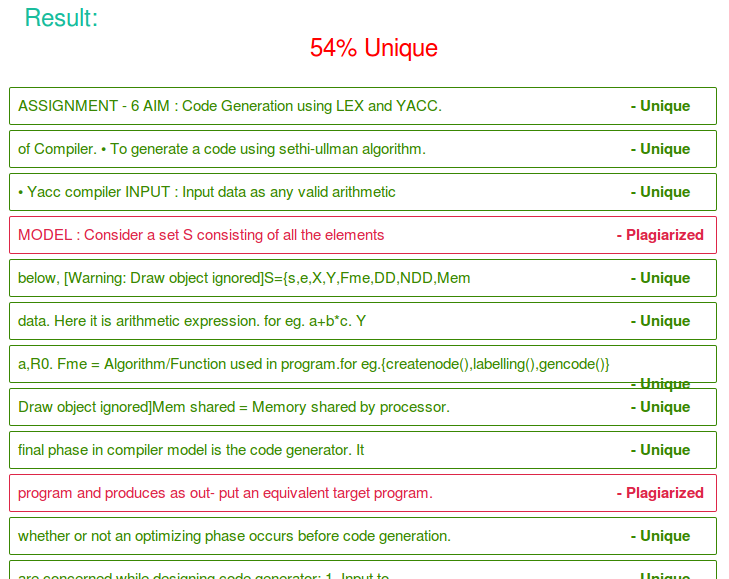
\includegraphics[height=5in,width=6in]{plagiarism6.png}
		\caption{Plagarism Checker www.smallseotools.com/plagarism-checker}
	\end{figure}
	\newpage
\end{document}

